\chapter{Specifying your geometry with a Z-Matrix}

A Z-Matrix is a convenient way to specify the geometry of a molecule or
crystal in terms of bond lengths, bond angles, and dihedral angles.
There are several styles of Z-matrix used in various programs,
\calcprog\ uses a format similar to that used in Gaussian.
This is intended to be a brief introduction to how a Z-matrix works.

If you already know how to use a Z-matrix, here's all you need to know
about the implementation in \calcprog:
\begin{itemize}
\item The first atom is put at the origin.
\item The second atom is put along the Z axis.
\item The third atom is in the XZ plane.
\item Dihedrals are evaluated using the right hand rule.
\end{itemize}

The easiest way to explain a Z-matrix is to show one and then explain
it, so that's what we'll do.  Before we start, however, we need to
briefly define a dihedral angle.  A dihedral is specified by 4
atoms, we'll call them A, B, C, and D.  The dihedral A--B--C--D is the
angle between the plane defined by A--B--C and the plane defined by
B--C--D.
Here's an alternative explanation: the dihedral A--B--C--D is the angle
between the lines C--D and B--A if you are looking down the line C--B.
There's one more piece of information we need to fully understand the
dihedral: there is a handedness associate with them.  If you think
about it, looking down the line C--B there are two different angles
between lines C--D and B--A: $\theta$ and 360-$\theta$.  The dihedrals
in \calcprog\ are defined using the right hand rule:  Take your right
hand and point the thumb down the line C--B, now align your fingers
with the line C--D, curling your fingers shows the direction in which
the dihedral angle is measured.
%
This is all about a million times easier to understand using a
picture, here's a picture demonstrating both views of dihedrals and
their handedness. 
%
\begin{center}
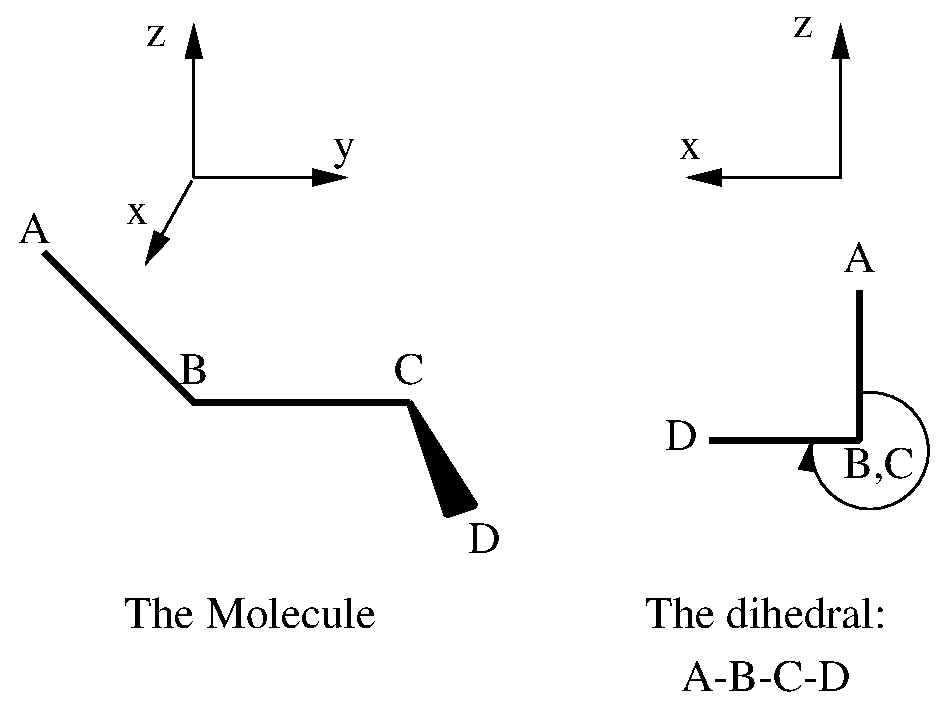
\epsfig{file=dihedral.eps,width=5.0in}
\end{center}
%

With that definition under our belt, here's the Geometry specification for a 
square pyramidal (CH$_3$)BiI$_4$ fragment, where the CH$_3$ group is
along the Z axis and the Bi and four I's lie in the XY plane:

\shrinkspacing
\begin{verbatim}
Geometry Z Matrix
9
1 Bi
2 C 1 2.1
3 I 1 2.7  2  90.0
4 I 1 2.7  2  90.0  3  90.0
5 I 1 2.7  2  90.0  3 180.0
6 I 1 2.7  2  90.0  3 270.0
7 H 2 1.1  1 109.5  3   0.0
8 H 2 1.1  1 109.5  3 120.0
9 H 2 1.1  1 109.5  3 240.0
\end{verbatim}
\resumespacing

Let's look at the first few entries in more detail.
\begin{enumerate}
\item The first atom is a Bi and it's placed at the origin.
Cartesian:  (0 0 0).  

\item Atom two is a C.  It's placed on the Z axis, 2.1 \AA\ away from
atom 1. Cartesian: (0 0 2.1).

\item Atom three is an I.  It's placed 2.7 \AA\ away from atom 1 and
the angle between atoms 3--1--2 in the XZ plane is 90.0 degrees.  
Cartesian: (2.7 0 0).

\item Atom four is an I.  It's placed 2.7 \AA\ away from atom 1, the
angle 4--1--2 is 90 degrees.  This angle puts us in the XY plane.  At
this point we know that atom 4 lies on a circle in the XY plane with
radius 2.7 \AA. The
dihedral 4--1--2--3 (90 degrees) tells us where on the circle we are. 
This dihedral is particularly easy to see:  if we look down the bond
2--1 (which is looking down the Z axis), the angle between the bond
3--1 and the bond 4--1 is 90 degrees.  So atom 4 lies on the Y axis.
Taking the right-handedness of dihedrals into account, we know that
atom 4 lies on the negative Y axis.  Cartesian (0 -2.7 0).

\item Atom five is an I.  It's 2.7 \AA\ away from atom 1, making an
angle of 90 degrees with 2 and a dihedral of 180 with 3.  This puts us
on the negative X axis.  Cartesian (-2.7 0 0).

\end{enumerate}

If you find the handedness of dihedrals confusing, just play around
with a couple of molecules defined using Z matrices, you'll get the
hang of it fairly quickly.

